\documentclass{article}
\usepackage{graphicx} % Required for inserting images
\usepackage{biblatex}
\usepackage{float}
\graphicspath{ {./imgs/} }
\addbibresource{proposal.bib}

\title{The effect of behavioral changes on the spread of COVID-19.}
\author{Ali Ali}
\date{September 2025}

\begin{document}

\maketitle
\section{Project Overview}
\subsection{Domain}
Our model's domain is epidemiology, specifically the study of how disease spreads.
\subsection{Problem Statement}
How do behavioral changes affect the spread of COVID-19? Are behavioral changes enough to eradicate COVID-19?
\subsection{Scope}
What will not be simulated:
\begin{itemize}
  \item An endemic model
  \item Population inflows and outflows
  \item Disease seasonality
  \item Usage of medical facilities
  \item Vaccination
  \item Age based components
\end{itemize}
What will be simulated:
\begin{itemize}
  \item An epidemic model  
  \item Pre-symptomatic infectious compartment
  \item Asymptomatic and symptomatic infectious compartments  
  \item Removed compartment
\end{itemize}

\section{System Description}
\subsection{System Components}
\begin{figure}[H]
  \center
  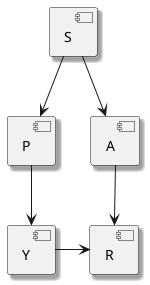
\includegraphics[scale=0.5]{A-1}
  \caption{Flowchart for the proposed model.}
\end{figure}

\begin{center}
\begin{tabular}{|l|l|} 
 \hline
 Variable & Description \\ [0.5ex] 
 \hline\hline
 S & Susceptible, can be infected \\
 \hline
 P & Pre-symptomatic, infectious without symptoms currently \\
 \hline
 A & Asymptomatic, infectious without symptoms forever \\
 \hline
 Y & Symptomatic, infectious with symptoms \\
 \hline
 R & Removed, recovered or dead \\
 \hline
\end{tabular}
\end{center}

The above model is derived from the standard SIR model. The Infectious component is divided into three compartments as each is likely to have a different effect on behavioral patterns, though pre-symptomatic and asymptomatic are likely to have the same effect but asymptomatic does not transition into symptomatic.

\subsection{System Dynamics}
\[
  \scalebox{2}{
  $S^' = - \frac{s(p + a + y)}{T} \beta S (\kappa _1 P + \kappa _2 A + \kappa _3 Y )$}
\]

\[
  \scalebox{2}{$
    P^' = \theta _1 \frac{s(p + a + y)}{T} \beta S (\kappa _1 P + \kappa _2 A + \kappa _3 Y) - \phi P
  $}
\]

\[
  \scalebox{2}{$
    A^' = \theta _2 \frac{s(p + a + y)}{T} \beta S (\kappa _1 P + \kappa _2 A + \kappa _3 Y) - \gamma A
  $}
\]

\[
  \scalebox{2}{$
    Y^' = \phi P - \gamma Y
  $}
\]

\[
  \scalebox{2}{$
    R^' = \gamma Y + \gamma A
  $}
\]
\begin{center}
\begin{tabular}{|l|l|} 
  \hline
  Symbol & Description \\ [0.5ex] 
  \hline\hline
  $s, p, a, y$ & rate of contact from component \\
  \hline
  $S, P, A, Y, R$ & rate of population of component \\
  \hline
  $T$ & $sS+ pP + aA + yY + R$ total rate of contact of components \\ 
  \hline
  $\beta$ & population rate of contact \\
  \hline
  $k_1, k_2, k_3$ & infection rate per contact \\
  \hline
  $\theta _1 , \theta_2$ & rate of susceptible to infectious class \\
  \hline
  $\phi$ & rate of pre-symptomatic to symptomatic \\
  \hline
  $\gamma$ & rate of recovery \\
  \hline
\end{tabular}
\end{center}
\subsection{Core Models and Algorithms}
\subsubsection{SIR Model}

The SIR model is a categorical model that can be used to model an epidemic by dividing a population into three categories, Susceptible, Infectious, and Recovered. Over time the population inside each category can be described with a set of differential equations:
\[
\frac{ds}{dt} = -\beta si
\]
\[
\frac{di}{dt} = \beta si - \gamma i 
\]
\[
\frac{dr}{dt} = \gamma i
\]

\begin{center}
  \begin{tabular}{|l|l|}
    \hline
    Symbol & Description \\ [0.5ex]
    \hline\hline
    $s, i, r$ & rate of population of component \\
    \hline
    $t$ & time \\
    \hline
    $\beta$ & rate of contact \\
    \hline
    $\gamma$ & rate of recovery \\
    \hline
  \end{tabular}
\end{center}
\cite{python}

\subsubsection{Behavioral change in populations}
A population demonstrates behavioral change during a pandemic by reducing their rate of contact. This effect can be dependent on which compartment an individual is in. It can be modeled by modifying the SIR differential equations into:
\[
  \frac{ds}{dt} = - \beta \frac{pq}{T}si
\]
\[
  \frac{di}{dt} = \beta \frac{pq}{T}si - \gamma I
\]

\begin{center}
  \begin{tabular}{|l|l|}
    \hline
    Symbol & Description \\ [0.5ex]
    \hline\hline
    $s, i $ & rate of population of component \\
    \hline
    $t$ & time \\
    \hline
    $\beta$ & rate of contact \\
    \hline
    $\gamma$ & rate of recovery \\
    \hline
    $p, q$ & change in rate of contact \\
    \hline
    $T$ & $ps + qi + r$ total rate of contact of components \\
    \hline
  \end{tabular}
\end{center}

\cite{behavior}
\subsection{Assumptions}
\begin{itemize}
\item The population will stay constant. 
\item The virus will not be affected by seasonal changes. 
\item The population will mix homogeneously.  
\item The population will not lose immunity. 
\item The virus will not mutate significantly.
\item Different infectious compartments will recover at the same rate.
\end{itemize}

\section{Implementation Approach}
\subsection{Programming Language}
The programming language to be used for this model will be Python for the following reasons:
\begin{itemize}
\item I have experience with Python.
\item All my references use Python.
\item Python is a popular language for modeling.
\end{itemize}

\subsection{Development Environment}
The python libraries used to develop this project will be:
\begin{itemize}
\item Pandas 
\item Matplotlib
\end{itemize}
Finally, the IDE used will be Emacs since I already have a python development environment setup.

\subsection{Simulation Type}
The behavioral change model will be a continuous model where the state of the population is dependent on time.

\subsection{Data Collection Plan}
The following metrics will be tracked:
\begin{itemize}
  \item Total number of infections
  \item Time until peak of the outbreak
  \item Peak number of infections
\end{itemize}


\section{Literature Review}
\subsection{\textit{Modeling and Simulation in Python}}
\subsubsection{Summary}
This source describes a model to simulate a "Freshman Plague" where 89 students arrive at a campus healthy while 1 student comes carrying some infectious disease.
The model is called the \textit{Kermack-McKendrick Model} which is a $SIR$ model where the population is divided into three categories, (S)upsceptible, (I)nfectious, and (R)ecoverd. The number of susceptible becoming infected is \[\beta siN\] per day, where $\beta$ is the contact rate, $s$ is the fraction of the population susceptible, $i$ is the fraction of the population infectious, and $N$ the population number. The number of infectious becoming recovered is \[\gamma iN\], where $y$ is the rate of recovery, $i$ is the number of infectious, and $N$ is the population number.
\cite{python}
\subsubsection{Adaption and Application}
An application for this paper with regards to our project is the component model it describes for epidemics. Specifically, the Kermack-McKendrick model which can be used to model the COVID-19 pandemic within a college campus. The SIR model and the two related equations will become the core part of our project.

\subsection{\textit{A simple model for behavior changes in epidemics}}
\subsubsection{Summary}
The above paper models the change in behavior that a population demonstrates during a pandemic. Specifically, it assumes that susceptible members during an pandemic decrease their rate of contact by a fraction $p$, $0 \le  p \le 1$, and that infectious members decrease their rate of contact by a fraction $q$, $0 \le q \le 1$. This model then gives a pair of difference equations to represent this change.
The first equation is \[S' = -\beta N\frac{pq}{T}SI\] where $S'$ is the change in Susceptible with respect to time, $\beta$ the rate of contact, $N$ the population, $p$ the fraction in change of contact for Susceptible, $p$ the fraction in change of contact for Infectious, $q$ the fraction in change of contact for Infectious, $T$ is $pS + qI + R$, $S$ the fraction of the population that is Susceptible, and $I$ the fraction of the population that is Infectious. 
The second equation is \[I' = \beta N \frac{pq}{T}SI-\alpha I\] where $I'$ is the change in Infectious with respect to time, $\alpha$ the rate of recovery, and $I$ the fraction of the population that is Infectious.
\cite{behavior}
\subsubsection{Application and Adaption}
This paper introduces a model that can be used to model self-isolation and social distancing for the COVID-19 pandemic. Our model will adapt the rate of contact by fractions and their difference equations for both Susceptible and Infectious.

\subsection{\textit{SEIR modeling of the COVID-19 and its dynamics}}
\subsubsection{Summary}
This paper describes a SEIR epidemic model which inputs parameters based on a particle swarm optimization algorithm of the Hubei, China province. The model separates the infectious compartment into two without intervention and with intervention parts. It is further described in Figure 1 and with the following set of difference equations:

\begin{figure}
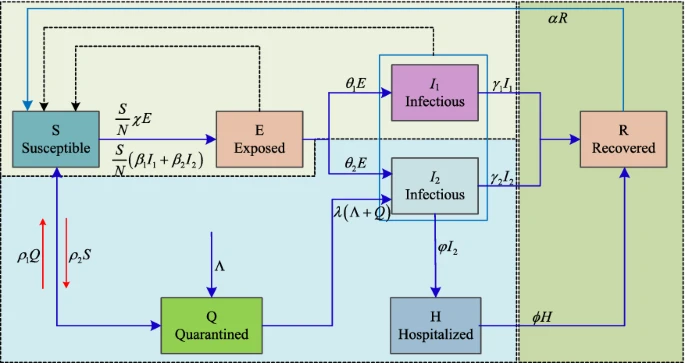
\includegraphics[scale=0.5]{dynamicmodel.png}
\caption{Flowchart model for the \textit{SEIR modeling of the COVID-19 and its dynamics}}
\end{figure}

\[\dot{S} = - \frac{S}{N} (\beta _1 I_1 + \beta _2 I_2 + \chi E) + \rho _1 Q - \rho _2 S + \alpha R\]
\[\dot{E} = \frac{S}{N} (\beta _1 I_1 + \beta _2 I_2 + \chi E) - \theta _1 E - \theta _2 E \]
\[\dot{I_1} = \theta _1 E - \gamma _1 I_1 \]
\[\dot{I_2} = \theta _2 E - \gamma _2 I_2 - \phi _2 I_2 - \phi I_2 + \lambda (\Lambda + Q) \]
\[\dot{R} = \gamma _1 I_1 + \gamma _2 I_2 + \Phi H - \alpha R \]
\[\dot{H} = \phi I_2 - \Phi I_2 H \]
\[\dot{Q} = \Lambda + \rho _2 S - \lambda (\Lambda + Q) - \rho _1 Q \]
\begin{tabular}{|l | l |} 
 \hline
 Variable & Description \\ [0.5ex] 
 \hline\hline
 $\alpha$ & Temporary immunity rate \\
 \hline
 $\beta _1 , \beta _2 $ & The contact and infection rate of transmission per contact from infected class \\
 \hline
 $\chi$ & Probability of transmission per contact from exposed individuals \\
 \hline
 $\theta _1 , \theta _2 $ & Transition rate of exposed individuals to the infected class \\
 \hline
 $\gamma _1 , \gamma _2 $ & Recovery rate of symptomatic infected individuals to recovered \\
 \hline
  $\phi$ & Rate of infectious with symptoms to hospitalized \\
  \hline
  $\Phi$ & Recovered rate of quarantined infected individuals \\
  \hline
  $\lambda$ & Rate of the quarantined class to the recovered class \\
  \hline
  $\rho _1 , \rho _2$ & Transition rate of quarantined exposed to quarantined infected to wider community \\
  \hline
  $\Lambda$ & External input from the foreign countries \\
  \hline
\end{tabular}
\cite{dynamic}
\subsubsection{Application and Adaption}
This paper describes a set of differential equations to reflect the different rate of infection of multiple infectious compartments. From it we will take $(\beta _1 I_1 + \beta _2 I_2 + \chi E)$ but replace it with three infectious components instead of two and one exposed component. This leads to $(\kappa_1 P + \kappa _2 A + \kappa_3 Y)$ where $P$ is pre-symptomatic, $A$ is asymptomatic, and $Y$ is symptomatic.


\subsection{Predicting the cumulative number of cases for the COVID-19 epidemic in China from early data}
\subsubsection{Summary}
This paper describes a SEIRU model in order to analyze the effects of the Chinese governments' imposed public policies in Wuhan from January 23, 2020 to January 29, 2020. The model consists of the following system of ordinary differential equations and is described in Figure 2.:

\[S^{'} (t) = - \tau (t)S(t)[I(t) + U(t)],\]
\[I^{'} (t) = \tau (t)S(t)[I(t) + U(t)] - \nu I(t), \]
\[R^{'} (t) = \nu _1 I(t) - \eta R(t), \]
\[U^{'} (t) = \nu _2 I(t) - \eta U(t) \]

\begin{figure}
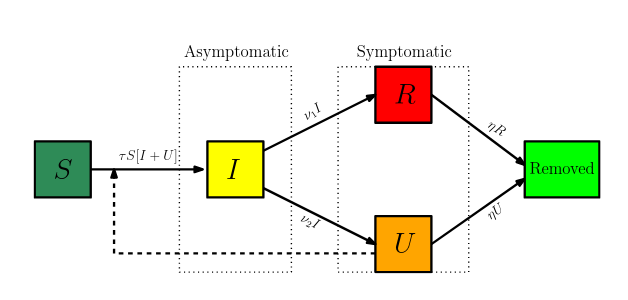
\includegraphics[scale=0.5]{cumulative.png}
\caption{Flowchart model for the \textit{Predicting the cumulative number of cases for the COVID-19 epidemic in China from early data} model}
\end{figure}

\begin{tabular}{|l | l |} 
  \hline
  Variable & Description \\ [0.5ex] 
  \hline\hline
  $S$ & Susceptible \\
  \hline
  $I$ & Asymptomatic \\
  \hline
  $R$ & Symptomatic reported \\
  \hline
  $U$ & Symptomatic unreported \\
  \hline
  $\tau (t)$ & Transmission rate at time t \\
  \hline
  $\nu _1 = f \nu$ & Rate of asymptomatic infectious becoming reported symptomatic \\
  \hline
  $\nu $ & Rate of asymptomatic to symptomatic \\
  \hline
  $\nu _2 = (1 - f) \nu$ & Rate of asymptomatic infectious becoming unreported symptomatic \\
  \hline
  $\eta $ & Rate of recovery \\
  \hline
\end{tabular}
\cite{cumulative}
\subsubsection{Application and Adaption}
The above paper describes a model that divides the infectious compartment to accurately model the COVID-19 epidemic. From it we will take the infectious compartments $I$ (Asymptomatic) , $R$ (Symptomatic Reported) , $U$ (Symptomatic Unreported) and remove the division of reported and unreported. Furthermore, we will add a separate asymptomatic compartment, since $I$ in the model is pre-symptomatic rather than true asymptomatic infection, which is important for our analysis.

\subsection{The role of asymptomatic and pre-symptomatic infection in SARS-CoV-2 transmission—a living systematic review}
\subsubsection{Summary}
The above study extracts data from multiple sources to determine the role of asymptomatic, pre-symptomatic, symptomatic infection in the transmission of SARS-CoV-2. Specifically, it estimates that asymptomatic viruses have a 1\% (95\% CI 0\%-2\%) infection rate, pre-symptomatic 7\% (95\% CI 3\% - 11\%), and symptomatic 6\% (95\% CI 5\% - 8\%).

\cite{review}
\subsubsection{Application and Adaption}
The above paper describes the important states of the COVID-19 epidemic and gives us an understanding of how to separate the infectious components of our project. Specifically, it tells us that asymptomatic, pre-symptomatic, and symptomatic states all have an important impact on the spread of COVID-19, which will be adapted into our model.

\section{Diagrams}
\begin{figure}[H]
  \center
  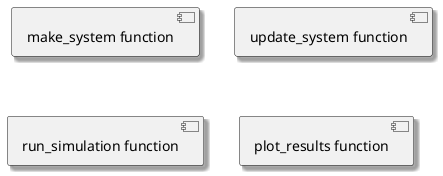
\includegraphics[scale=0.5]{A-2}
  \caption{Class Diagram}
\end{figure}

\begin{figure}[H]
  \center
  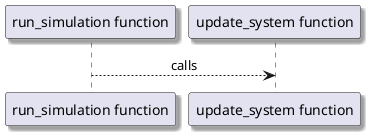
\includegraphics[scale=0.5]{A-3}
  \caption{Activity Diagram}
\end{figure}


\newpage
\printbibliography
\end{document}

